\documentclass[dvipsnames,mathserif]{beamer}
\setbeamertemplate{footline}[frame number]
\setbeamercolor{footline}{fg=black}
\setbeamerfont{footline}{series=\bfseries}
\usepackage{tikz}
\usepackage{xcolor}
\usepackage{graphicx, setspace, appendix, mathrsfs, amsmath, amsfonts,caption, mathtools}
\usepackage[english]{babel}
%\usetheme{Frankfurt}%1
\usetheme{Darmstadt}%1

% for RTL liste
\makeatletter
\newcommand{\RTListe}{\raggedleft\rightskip\leftm}
\newcommand{\leftm}{\@totalleftmargin}
\makeatother

% RTL frame title
\setbeamertemplate{frametitle}
{\vspace*{-1mm}
  \nointerlineskip
    \begin{beamercolorbox}[sep=0.3cm,ht=2.2em,wd=\paperwidth]{frametitle}
        \vbox{}\vskip-2ex%
        \strut\hskip1ex\insertframetitle\strut
        \vskip-0.8ex%
    \end{beamercolorbox}
}
% align subsection in toc
\makeatletter
\setbeamertemplate{subsection in toc}
{\leavevmode\rightskip=5ex%
  \llap{\raise0.1ex\beamer@usesphere{subsection number projected}{bigsphere}\kern1ex}%
  \inserttocsubsection\par%
}
\makeatother

% RTL triangle for itemize
\setbeamertemplate{itemize item}{\scriptsize\raise1.25pt\hbox{\donotcoloroutermaths$\blacktriangleleft$}} 

%\setbeamertemplate{itemize item}{\rule{4pt}{4pt}}

\defbeamertemplate{enumerate item}{square2}
{\LR{
    %
    \hbox{%
    \usebeamerfont*{item projected}%
    \usebeamercolor[bg]{item projected}%
    \vrule width2.25ex height1.85ex depth.4ex%
    \hskip-2.25ex%
    \hbox to2.25ex{%
      \hfil%
      {\color{fg}\insertenumlabel}%
      \hfil}%
  }%
}}

\setbeamertemplate{enumerate item}[square2]
\setbeamertemplate{navigation symbols}{}


\titlegraphic { 
\begin{tikzpicture}[overlay,remember picture, opacity=0.1,]
\node[] at (0, 2.9){
};\end{tikzpicture}}
\setbeamertemplate{caption}[numbered]
\begin{document}

\rightskip\rightmargin
\title{A flexible approach to parametric inference in nonlinear and time varying time series models }
\author{Gary Koop, Simon Potter (2010)}


%\institute{Boston College}
\footnotesize{\date{\today }


\begin{frame}
\maketitle
\end{frame}


%
\footnotesize \tableofcontents
%
\section{Motivation}
\begin{frame}{Motivation}
    \begin{itemize}
        \item Monetary policy rules have changed over time?
        \item For researchers working with macroeconomic and financial data, there is great interest in investigating whether structural breaks and regime-switching behavior occurs in the conditional mean, $E(y_t|T_{t-1})$, and the conditional variance, $var(y_t|T_{t-1})$.
        \item Models that are nonlinear or exhibit structural breaks or time variation in parameters.
        \item The set of possible models is huge. Data mining issue.
        \item Can we develop a flexible parametric model which nests almost all of these specifications?
    \end{itemize}  
\end{frame}


\section{Literature Review}
\begin{frame}{Literature Review}
    \begin{itemize}
        \item Structural break or time varying parameter models:\\
        Cogley and Sargent (2001, 2005), Boivin and Giannoni (2006), Primiceri (2005)
        \item Regime-switching models:\\
        Sims and Zha (2006), Koop and Potter (2006)
        \item Flexible parametric modeling:\\
        Hamilton (2001, 2003), Lundbergh et al. (2003), Bec et al. (2008), Giordani et al. (2007)
    \end{itemize}
\end{frame}

\section{Model}
\begin{frame}{Model}
    \begin{itemize}
        \item TVP written in state space form:\\
            \begin{align}
            y_t &= \theta_tx_t + \varepsilon_t\\
            \theta_t &= \theta_{t-1} + \nu_t
            \end{align}
        $\varepsilon_t$ is $i.i.d.$ $N(0,\sigma_\epsilon^2) $and $\nu_t$ is $i.i.d.$ $N(0,\sigma_\nu^2)$ - assume homoskedasticity in this simple case, include volatility issues in the general model.\\
        \item Add stochastic volatility to the measurement equation:\\
            \begin{align*}
            \varepsilon_t &= \xi_t exp\left(\frac{1}{2}\alpha_t\right)\\
            \xi_t &\sim N(0,1)\\
            \alpha_t &= \alpha_{t-1} + \eta_t\\
            \eta_t &\sim N(0, \sigma_\eta^2)
            \end{align*}
        
    \end{itemize}

\end{frame}
\begin{frame}{Model}
    \begin{itemize}
        \item The role of the distance function
            \begin{align}
            y_t &= \theta_ty_{t-1} + \varepsilon_t\\
            \theta_t &= \theta_{t-1} + d(t,t-1)\nu_t
            \end{align}
        \item links bwtween this framework with other time series models\\
        \begin{itemize}
            \item If $d(t,t-1) = 0$ $\rightarrow$ standard linear AR model
            \item If $d(t,t-1) = 1$ $\rightarrow$ TVP model as in Koop and Potter (2001)
            \item If $d(t,t-1) = 1$ if $t=\tau$ and $d(t,t-1) = 0$ otherwise, then $\theta_1 = \cdots = \theta_{\tau-1}$ and $\theta_{\tau} = \cdots = \theta_T$ $\rightarrow$ model with a single structural break at $\tau$
            \item Add a second breakpoint $\rightarrow$ model with two structural breaks
            \item $\cdots$ 
        \end{itemize}
    \end{itemize}
\end{frame}
\begin{frame}{Model}
    \begin{itemize}
        \item The role of hypothetical data reordering
            \begin{align}
                y_s &= \theta_sx_s + \varepsilon_s\\
                \theta_s &= \theta_{s-1} +  d(z_s, z_{s-1})\nu_s
                \end{align}
                where $z_t$ is an exogenous index variable, $\gamma$ define the ordering of the data according to $z_t$ and $s$ is the index under the new ordering
        \item Links between this framework with other time series models
        \begin{itemize}
            \item If $z_t = y_{t-1}$ (then $\gamma$ orders the data based on last period's $y$), define $d(z_s,z_{s-1}) = 1$ if $z_{s-1} < \tau$ and $z_s \geq \tau $ and $d(z_s,z_{s-1}) = 0$ otherwise $\rightarrow$ two-regime TAR model
                \begin{align*}
                y_t &= \theta_1x_t + \varepsilon_t \; if\,y_{t-1} <\tau\\
                y_t &= \theta_2x_t + \varepsilon_t \; if\,y_{t-1} \geq\tau
                \end{align*}
        \end{itemize}
    \end{itemize}
\end{frame}

\begin{frame}{Model}
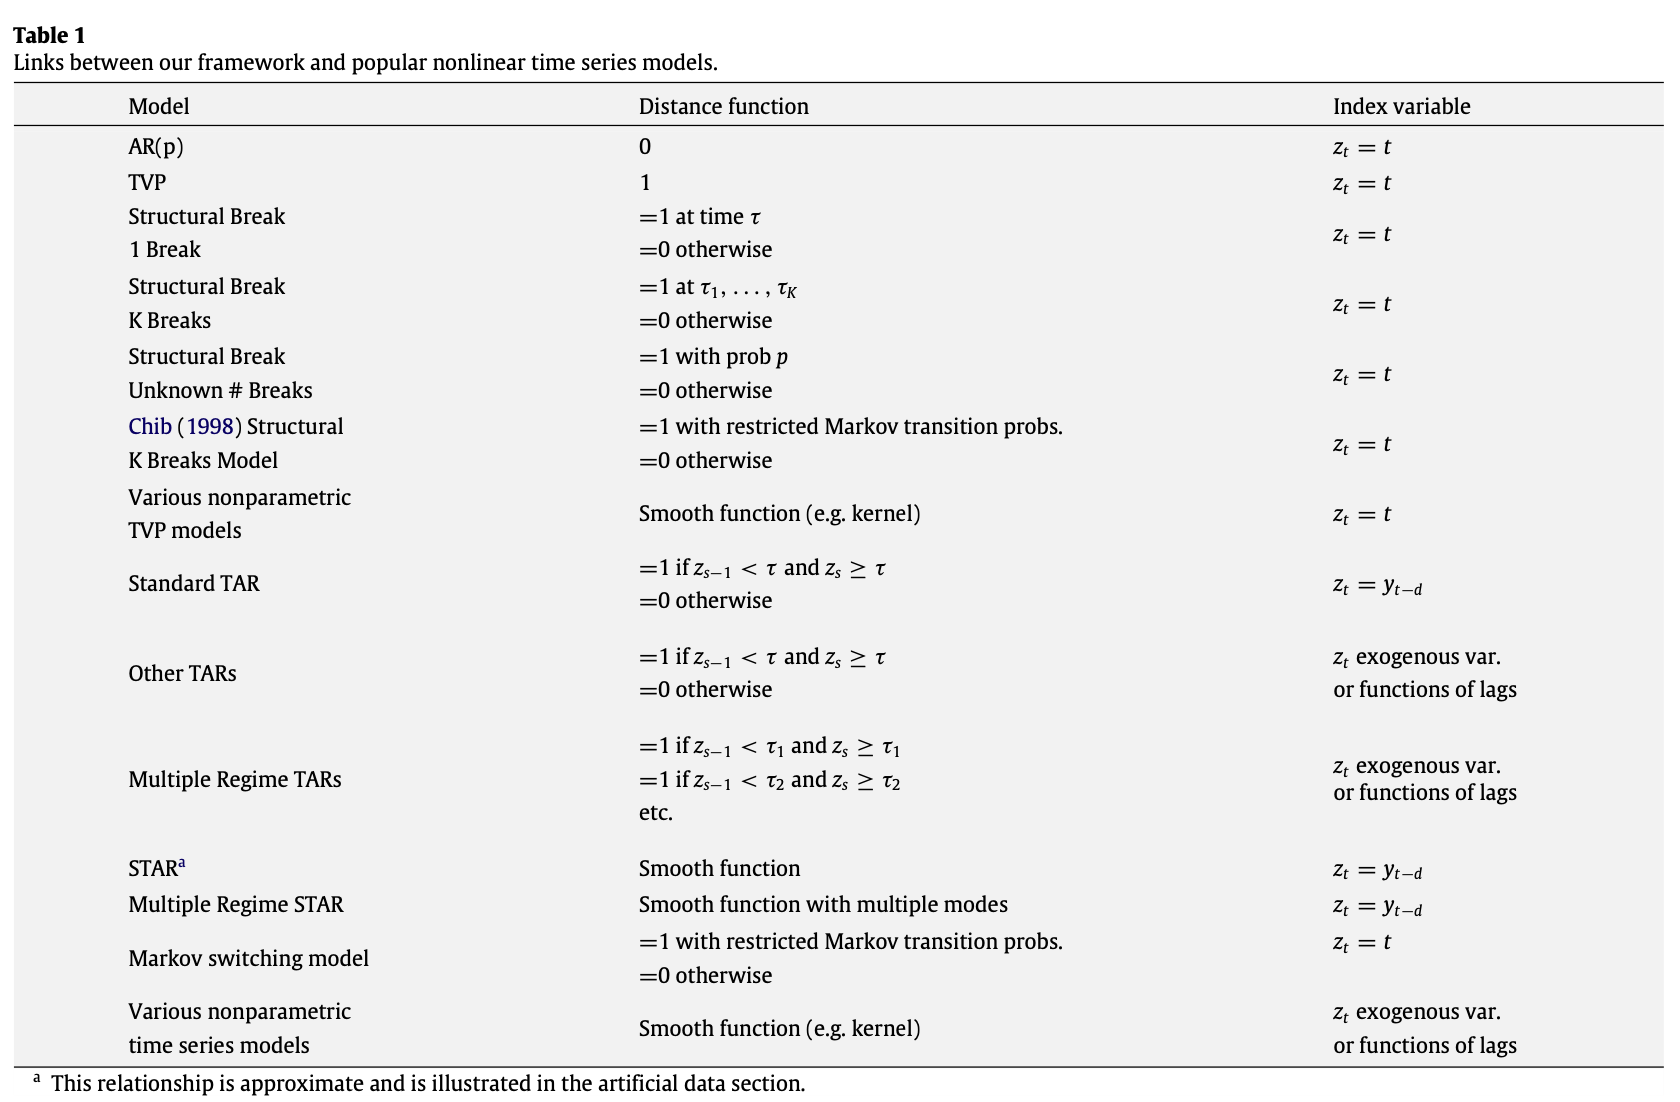
\includegraphics[width = 0.9\textwidth]{model.png}
\end{frame}

\section{Empirical work}
\begin{frame}{Empirical work}
    \begin{itemize}
        \item Artificial data
        \item Empirical illustrations using real GDP growth
        \item The oil price and GDP growth
    \end{itemize}
\end{frame}

\section{Discussion}
\begin{frame}{Discussion}
    \begin{itemize}
        
        \item This model nests virtually every popular model in the regime-switching and structural break literatures, including everything from abrupt change models (e.g. threshold autoregressive models or structural break models such as Bai and Perron (1998)) to those which allow gradual evolution of parameters (e.g. smooth transition autoregressive models or TVP models such as Primiceri (2005)).
        \item This model adds two simple concepts, hypothetical reordering and distance, to a standard state space framework.
        \item Retain the state space framework, bayesian econometric methods are relatively straightforward drawing on the existing literature. 
    \end{itemize}
\end{frame}



\end{document}